\section{Introduction}
\label{sec:intro}

Multimodal Social Event Detection (SED) aims to partition streams of short, noisy user-generated text--image posts into coherent real-world event clusters~\cite{lin2024ned,han2026kqgnn,yang2026seinevent}. Because social posts frequently omit explicit named entities or background context---writing only generic reactions such as \emph{``Evacuation of detainees from the stadium after the explosion!''} or \emph{``It took volunteers 4 days to clear our section of the road''}---attaching a photo can visually supply missing landmarks, uniforms, damaged infrastructure, or event signage that unifies posts missed by text encoders. At the same time, social streams contain high-frequency viral memes, reaction GIFs, news outlet logos, off-topic selfies, and cross-incident attachments that pull semantically unrelated threads together under shared visual templates. Deciding \emph{when images disambiguate events} rather than corrupting text clusters is therefore central to reliable multimodal SED.

\paragraph{The Hidden Chronological Shortcut and Static Heuristic Traps.}
Unfortunately, evaluating multimodal SED directly on standard chronological streams obscures this trade-off. When benchmark events are chronologically separated in calendar time---such as the 40-event \texttt{NED} corpus~\cite{lin2024ned} spanning 2011--2021---a trivial temporal partition splitting the stream at 72-hour gaps already achieves $B^3\text{-}F_1 = 0.9900$ (Precision $0.9810$, Recall $0.9992$) before examining a single pixel or word. Under naive chronological clustering, almost any time-windowed multimodal model inherits near-perfect scores from calendar separation alone, masking how images behave when multiple same-topic events compete concurrently.

Even when researchers intuit that ``visual noise'' exists, two common simplifications fail in practice:
\begin{enumerate}
    \item \textbf{Naive Multimodal Fusion Assumes Images Rarely Harm:} Concatenating or summing visual similarities without reliability gating rescues ambiguous posts, but leaves both graph clustering and Vision-Language Models (VLMs) defenseless when competing events share visually plausible imagery (e.g., two hurricanes producing indistinguishable flood photos, or two disasters mixed via cross-event image swap). Under a controlled $30\%$ competing-image corruption stress test on \texttt{NED}, naive multi-view clustering plunges by $-13.35\text{ pp}$ (validation) and $-8.11\text{ pp}$ (holdout) in Event Macro-$B^3$, performing \emph{worse} than discarding images altogether.
    \item \textbf{Static Text-Dispersion Penalties Misclassify Multi-Angle Reporting:} A tempting unsupervised signal---which we formalize and audit as Cross-Neighbor Text Dispersion (\texttt{CNTD-Raw})---downweights any image whose visual neighbors accompany diverse caption texts, assuming it must be a generic meme. In reality, one genuine breaking-news photograph is routinely captioned from diverse angles (evacuation orders, traffic closures, casualty counts, relief appeals). Penalizing text dispersion blindly destroys legitimate visual rescues ($96 \to 59$ in paired CLIP scoring; $17 \to 7$ in VLM auditing; $-4.80\text{ pp}$ Macro-$B^3$ in 2D-SE clustering) while leaving unique out-of-context distractors (\texttt{Visual-IDF} $= 1.0$) untouched.
\end{enumerate}

\paragraph{Causal Diagnosis Meets Two-Stage Evidence Gating.}
To isolate genuine visual utility without calendar shortcuts, we construct an event-relative concurrent alignment ($\tau^{\text{rel}}_i = \tau_i - \min_{j \in E(i)} \tau_j$) across strictly separated event splits (`8` development, `8` validation, `24` unseen holdout) with all event titles and dates stripped. On the 8-event development split, a paired three-condition counterfactual audit (\texttt{Text-Only}, \texttt{Orig-Img}, \texttt{Mismatched-Img}) using both frozen CLIP~\cite{radford2021clip} ($n=1{,}527$ novel non-duplicate query images, $\mathrm{dHash} > 6$) and \texttt{Qwen/Qwen3-VL-8B-Instruct}~\cite{bai2025qwen3vl} ($360/360$ audited calls) empirically validates the dual-regime hypothesis: visual value is \emph{competitor-conditioned} and requires separating frequency suppression (graph level) from cross-modal semantic conflict detection (reasoning level).

Guided directly by Gate~B, we propose \textbf{Evid-MSED} (Figure~\ref{fig:overview}). In Stage~1 (zero API cost), chunked \texttt{Visual-IDF} downweights repeated templates while a corrected soft-imputation scheme fills missing-image posts from reliable neighborhood consensus---fixing a mathematical inconsistency ($\delta_i \delta_j = 0$) from prior missing-modality graph designs---before minimizing exact 2D Structural Entropy (2D-SE)~\cite{li2016structural,cao2024hisevent}. In Stage~2, a budgeted multimodal mesoscopic seam router~\cite{bai2025qwen3vl,wang2025cequel} pairs fragmented cluster siblings (\texttt{MM\_MERGE\_PAIR}) and low-conductance minority pockets (\texttt{MM\_SPLIT\_SEAM}), queries \texttt{Qwen/Qwen3-VL-8B-Instruct} with Visual-IDF-weighted representative images and anonymized medoid texts, and gates execution on explicit \texttt{visual\_discriminative} and \texttt{visual\_conflict\_with\_text} predictions before direct split-then-union-find editing.

\paragraph{Contributions.}
This paper makes four empirically grounded contributions:
\begin{itemize}
    \item \textbf{Causal Quantification of Visual Rescue vs.\ Mislead Beyond Time Shortcuts:} Removing calendar separation on \texttt{NED} and deduplicating query images ($\mathrm{dHash} > 6$), we deliver paired three-condition counterfactual audits across both CLIP ($n=1{,}527$) and \texttt{Qwen/Qwen3-VL-8B-Instruct} ($360$ live calls, $332{,}778$ tokens), refuting the \texttt{CNTD-Raw} dispersion heuristic and proving that cross-modal conflict gating boosts VLM original accuracy to $85.00\%$ ($0$ misleads vs.\ $7$) while slashing competing-mismatch flips from $77$ to $0$--$5$.
    \item \textbf{Unified Missing-Modality Soft Imputation for 2D-SE:} We eliminate the degenerate missing-modality indicator factor $\delta_i \delta_j$ in multi-view structural entropy graphs (Proposition~\ref{prop:soft_impute}), proving consistent Event Macro-$B^3$ improvements across all five tested splits and corruption settings ($+0.68$ to $+3.27\text{ pp}$).
    \item \textbf{Conflict-Gated Multimodal Mesoscopic Adjudication (\texttt{Evid-MSED}):} Under an immutable SHA-256 frozen protocol on the 24-event unseen \texttt{NED} holdout stream ($11{,}955$ posts, $9{,}311/9{,}311$ decoded images, $360/360$ clean + $119/120$ stress VLM calls), Stage~1 lifts Clean Macro-$B^3$ by $+6.38\text{ pp}$ (AMI $+3.84\text{ pp}$) over text-only 2D-SE and holds $+4.18\text{ pp}$ above collapsing naive fusion under $30\%$ corruption; Stage~2 delivers $19.45$ (Val Clean) and $24.63$ (Holdout $K=60$) net unqueried posts fixed per call ($5.6\times$ blind VLM leverage at $K=180$) and $100\%$ stress merge precision ($1/0$).
    \item \textbf{Candid Head/Medium/Tail Failure Analysis:} Stratified $B^3$ decomposition across all 24 holdout events reveals that while Stage~2 drives Head-event $B^3$-$F_1$ from $0.3703 \to 0.4545 \to 0.5008$ ($+13.05\text{ pp}$), just two size-asymmetric hard union-find merge false positives touching tail events ($<200$ posts) account for aggregate Macro-$B^3$ flattening, pointing directly to size-guarded graph surgery as future work.
\end{itemize}

\begin{figure*}[t]
  \centering
  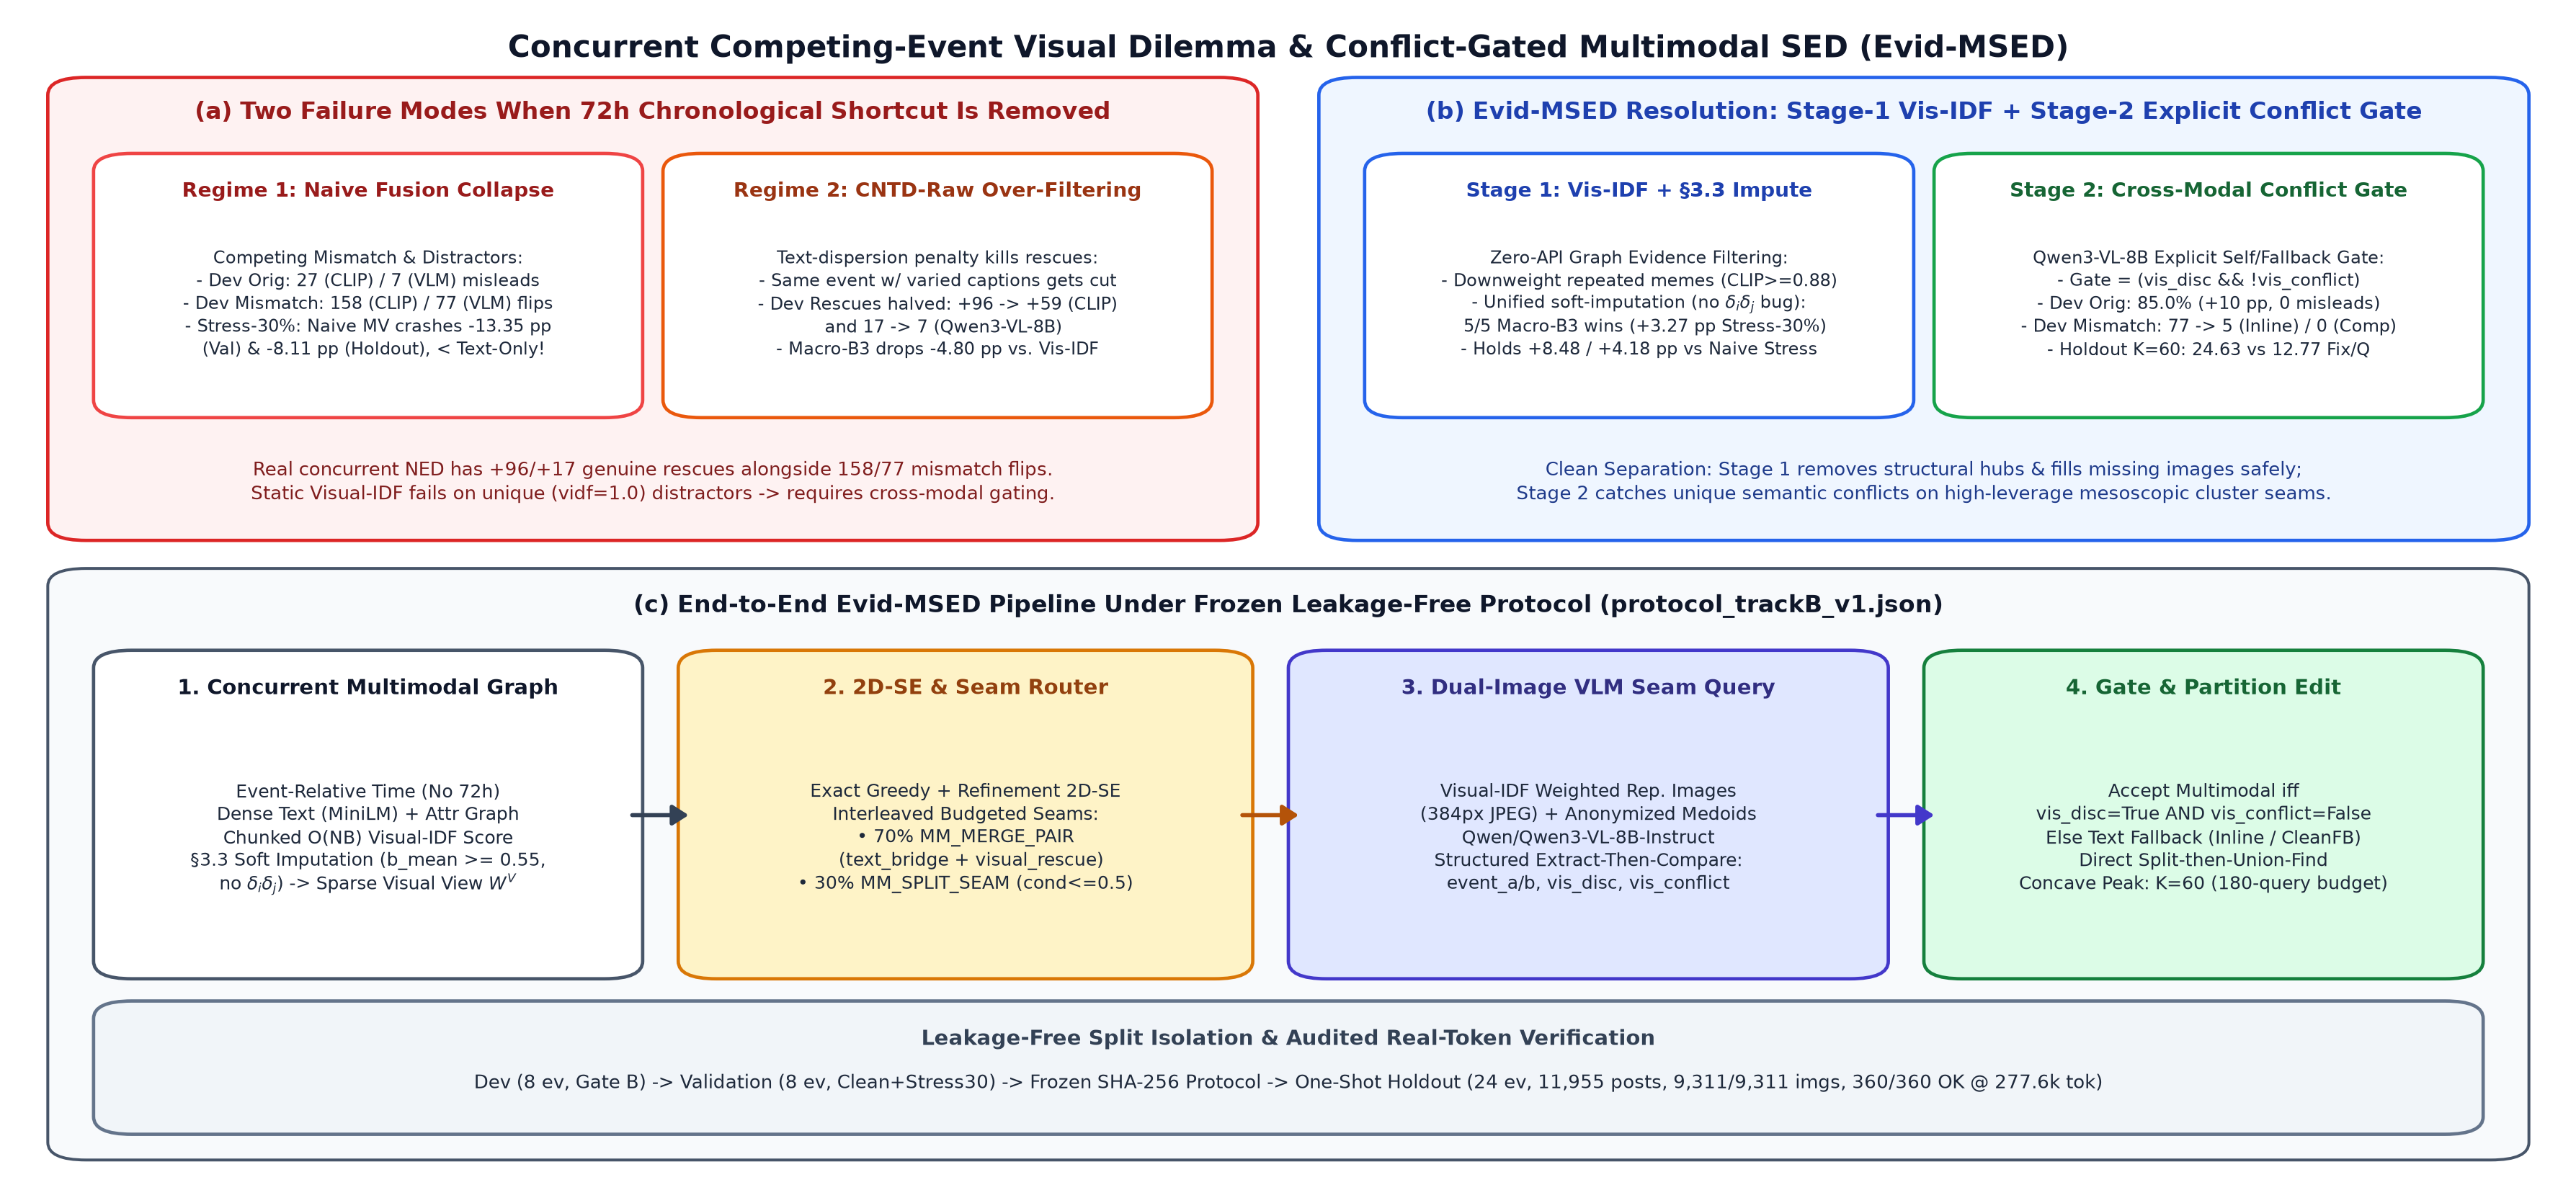
\includegraphics[width=0.98\textwidth]{figures/fig_overview_evid_msed.png}
  \caption{Overview of the concurrent visual evidence dilemma on time-shortcut-free streams (top) and our frozen two-stage \textbf{Evid-MSED} pipeline (bottom) combining chunked \texttt{Visual-IDF} MV-2DSE with conflict-gated mesoscopic VLM seam adjudication.}
  \label{fig:overview}
\end{figure*}
